% FAIR Data Curation for Our Lab -- Beamer version (generated from deck_spec.py)
% Build: latexmk -xelatex talk.tex     Notes PDF: uncomment the pgfpages line below.
\documentclass[aspectratio=169]{beamer}
\geometry{paperwidth=10in,paperheight=5.625in}
\usetheme{ISU}
% \usepackage{pgfpages}\setbeameroption{show notes on second screen=right}
\setlength{\fboxsep}{0pt}\setlength{\fboxrule}{0.5pt}
\newcommand{\imgframe}[1]{{\color{isuCoolGray!70}\fboxsep0pt\fboxrule0.5pt\fbox{#1}}}
\begin{document}

{\setbeamertemplate{footline}{}\begin{frame}[plain]
\begin{tikzpicture}[remember picture,overlay]\fill[isuRed] (current page.north west) rectangle ++(10in,-0.12in);\end{tikzpicture}
\at{0.69}{0.8}{{\fontsize{10.5}{12}\selectfont\color{isuRule}\bfseries GROUP MEETING  ·  DATA STEWARDSHIP}}
\begin{tikzpicture}[remember picture,overlay]\node[anchor=south west,inner sep=0,text width=8.62in,font=\headfont\fontsize{32}{36}\selectfont,text=isuRed] at ([xshift=0.69in,yshift=-1.9in]current page.north west) {FAIR Data Curation for Our Lab};\draw[isuRule,line width=1.5pt] ([xshift=0.69in,yshift=-2.02in]current page.north west) -- ([xshift=9.31in,yshift=-2.02in]current page.north west);\end{tikzpicture}
\at{0.69}{2.15}{\begin{minipage}{8.62in}\fontsize{17}{21}\selectfont Making our phenotyping data findable, usable, and ready for USDA and NSF data sharing\end{minipage}}
\panel{0.69}{3.05}{2.02}{1.45}{isuTintBlue}{{\headfont\fontsize{38}{40}\selectfont\color{isuRed}F}\par\vspace{2pt}{\fontsize{13}{15}\selectfont\color{isuNavy}\bfseries Findable}\par{\fontsize{10.5}{13}\selectfont someone can locate it}}
\panel{2.89}{3.05}{2.02}{1.45}{isuTintIce}{{\headfont\fontsize{38}{40}\selectfont\color{isuRed}A}\par\vspace{2pt}{\fontsize{13}{15}\selectfont\color{isuNavy}\bfseries Accessible}\par{\fontsize{10.5}{13}\selectfont they can open it}}
\panel{5.09}{3.05}{2.02}{1.45}{isuTintGreen}{{\headfont\fontsize{38}{40}\selectfont\color{isuRed}I}\par\vspace{2pt}{\fontsize{13}{15}\selectfont\color{isuNavy}\bfseries Interoperable}\par{\fontsize{10.5}{13}\selectfont their tools can read it}}
\panel{7.29}{3.05}{2.02}{1.45}{isuTintGray}{{\headfont\fontsize{38}{40}\selectfont\color{isuRed}R}\par\vspace{2pt}{\fontsize{13}{15}\selectfont\color{isuNavy}\bfseries Reusable}\par{\fontsize{10.5}{13}\selectfont they know how, and may}}
\at{0.69}{4.85}{\begin{minipage}{8.62in}\fontsize{11}{13}\selectfont Zaki Jubery  ·  Agricultural \& Biosystems Engineering and Translational AI Center  ·  Iowa State University\end{minipage}}
\note{Today is about one practical question: if you left the lab tomorrow, could someone else find, open, understand, and legally reuse your data? FAIR is the name for the four things that make that true: Findable, Accessible, Interoperable, Reusable. I will keep it hands-on. By the end you will have a folder layout, a naming rule, a short list of formats, and a tool that does most of the work for you. About 20 minutes, then we try it on one real dataset.}\end{frame}}

\begin{frame}
\isutitle[21]{The dataset that disappeared}
\at{0.69}{1.4}{\begin{minipage}[t]{4.3in}\raggedright\fontsize{12.5}{16.25}\selectfont{}\color{isuBody}A student finishes a UAV-LiDAR maize project. The paper says {\color{isuInk}\bfseries "data available upon request."}\par\vspace{3.75pt}
Two years later a reviewer asks for it. The student has graduated.\par\vspace{3.75pt}
The shared link opens a folder like the one on the right.\par\vspace{3.75pt}
\par\vspace{6.25pt}{\color{isuNavy}\bfseries Questions nobody can answer now}\par\vspace{1pt}
\begin{itemize}\setlength{\itemsep}{3.75pt}\setlength{\leftmargini}{1.1em}
\item Which flight date is each cloud from?
\item Which plot and genotype is which?
\item Which coordinate system? Which software?
\item Who is allowed to reuse it?
\end{itemize}\end{minipage}}
\panel{5.25}{1.45}{4.06}{2.45}{isuCode}{{\ttfamily\fontsize{11.5}{14.95}\selectfont{}\color{isuInk}final\_v3\_REAL/\\\hphantom{0}\hphantom{0}cloud\_merged\hphantom{0}FINAL.las\\\hphantom{0}\hphantom{0}lidar\_aug2\_v3\_REAL.laz\\\hphantom{0}\hphantom{0}lidar\_aug2\_v3\_REAL\hphantom{0}(1).laz\\\hphantom{0}\hphantom{0}plot\hphantom{0}map\hphantom{0}FINAL.xlsx\\\hphantom{0}\hphantom{0}\textasciitilde{}\$plot\hphantom{0}map\hphantom{0}FINAL.xlsx\\\hphantom{0}\hphantom{0}Untitled.ipynb\\\hphantom{0}\hphantom{0}Untitled1.ipynb\\\hphantom{0}\hphantom{0}New\hphantom{0}folder/IMG\_4521.HEIC}}
\statement{0.69}{4.45}{8.62}{0.58}{\fontsize{14}{18.2}\selectfont{}The data still exists. It is just useless without the context that lived in one person's head.}
\note{Let me start with a story most of us have lived. A student finishes a drone LiDAR project. The paper says data available upon request. Two years later a reviewer or a new student asks for it. The person who made it is gone. The folder looks like this: final, v3, REAL, copy one. Nobody knows which flight each file came from, which plots are which genotypes, or what coordinate system the points are in. The files are not lost. The context is lost. FAIR is the habit of writing that context down while you still remember it.}\end{frame}

\begin{frame}
\isutitle[21]{Why now: our funders require it}
\at{0.69}{1.35}{\imgframe{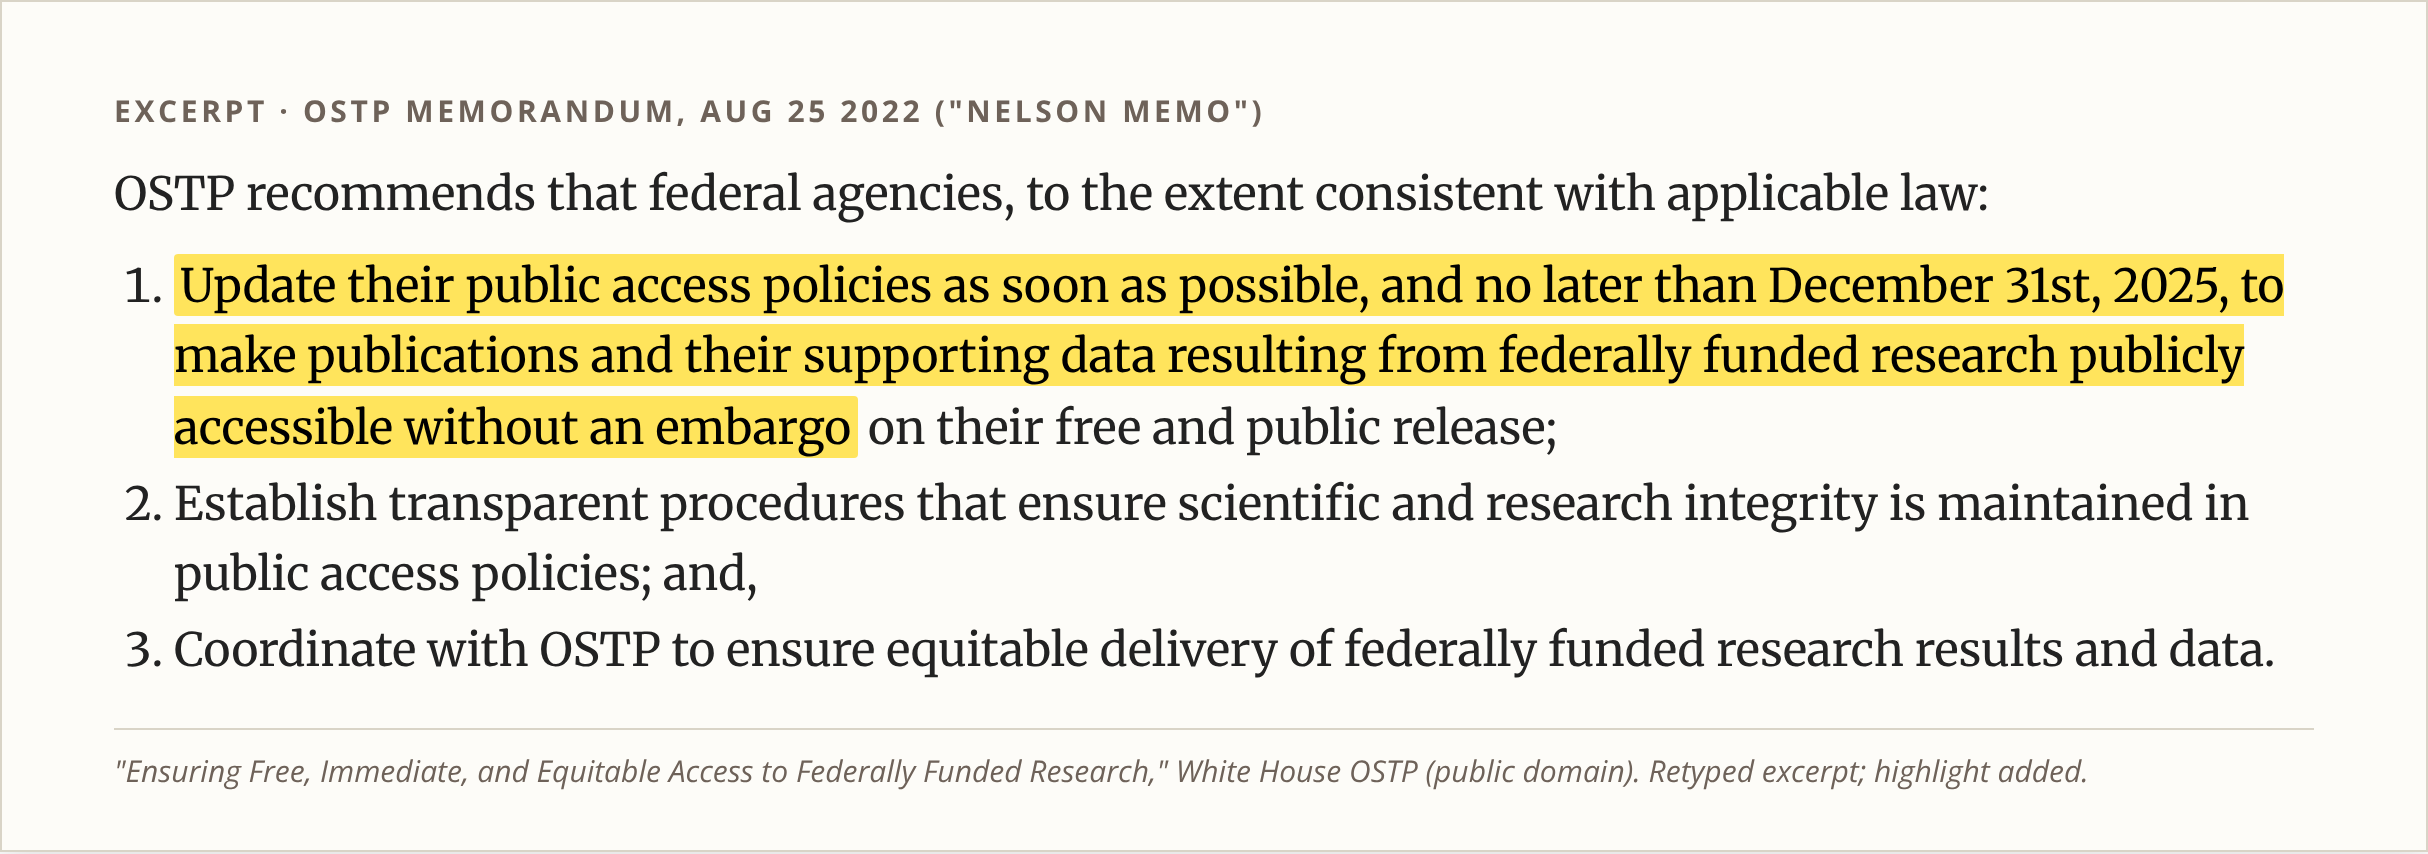
\includegraphics[width=6in,height=2.11038in]{img/excerpt_nelson.png}}}
\panel{6.95}{1.35}{2.36}{2.11}{isuPanel}{\raggedright{\fontsize{12.5}{16.25}\selectfont{}\color{isuRed}\bfseries €10.2 billion / year}\par\vspace{3pt}{\fontsize{11}{14.3}\selectfont{}\color{isuBody}Minimum yearly cost of non-FAIR research data to the EU economy (European Commission / PwC, 2018).}}
\panel{0.69}{3.65}{2}{1.38}{isuTintBlue}{\raggedright{\fontsize{12}{15.6}\selectfont{}\color{isuNavy}\bfseries Aug 2022}\par\vspace{3pt}{\fontsize{10.5}{13.65}\selectfont{}\color{isuBody}OSTP "Nelson memo": papers {\color{isuInk}\bfseries and supporting data}, no embargo}}
\panel{2.897}{3.65}{2}{1.38}{isuTintIce}{\raggedright{\fontsize{12}{15.6}\selectfont{}\color{isuNavy}\bfseries Dec 2024}\par\vspace{3pt}{\fontsize{10.5}{13.65}\selectfont{}\color{isuBody}Agencies publish new public-access policies}}
\panel{5.103}{3.65}{2}{1.38}{isuTintGreen}{\raggedright{\fontsize{12}{15.6}\selectfont{}\color{isuNavy}\bfseries Dec 2025}\par\vspace{3pt}{\fontsize{10.5}{13.65}\selectfont{}\color{isuBody}Deadline for the new policies to take effect (USDA, NSF, NIH…)}}
\panel{7.31}{3.65}{2}{1.38}{isuTintGray}{\raggedright{\fontsize{12}{15.6}\selectfont{}\color{isuNavy}\bfseries 2026}\par\vspace{3pt}{\fontsize{10.5}{13.65}\selectfont{}\color{isuBody}NeurIPS dataset track requires Croissant + Responsible-AI metadata}}
\note{Why does this matter now and not ten years ago? Because it became a rule. In August 2022 the White House science office told every federal agency, including USDA and NSF, to make publications and the data behind them public with no embargo. The highlighted line is the key part. Agencies had to publish new policies by the end of 2024 and put them in effect by the end of 2025. So every grant we write from here on needs a real data management plan, and reviewers will check it. Machine learning venues are doing the same thing: NeurIPS now requires a Croissant metadata file for dataset papers. And the cost of not doing this is large. The European Commission estimated at least 10 billion euros a year.}\end{frame}

\begin{frame}
\isutitle[21]{FAIR is a library catalog for data}
\at{0.69}{1.4}{{\fontsize{11.5}{14.95}\selectfont{}\renewcommand{\arraystretch}{1.3}\setlength{\tabcolsep}{0.06in}\arrayrulecolor{isuTintBlue}\begin{tabular}{>{\raggedright\arraybackslash}p{1.43in}>{\raggedright\arraybackslash}p{2.88in}>{\raggedright\arraybackslash}p{3.95in}}\rowcolor{isuNavy}\textcolor{white}{\bfseries Letter} & \textcolor{white}{\bfseries In a library} & \textcolor{white}{\bfseries In our lab}\\
\rowcolor{white}\textcolor{isuNavy}{{\color{isuInk}\bfseries F} Findable} & Call number + catalog card & A {\color{isuInk}\bfseries DOI} (permanent ID) + rich metadata in a searchable repository\\
\rowcolor{isuCode}\textcolor{isuNavy}{{\color{isuInk}\bfseries A} Accessible} & Clear borrowing rules; the card stays even if the book is lost & Download over HTTPS; login allowed; metadata stays online\\
\rowcolor{white}\textcolor{isuNavy}{{\color{isuInk}\bfseries I} Interoperable} & Written in a language readers know & Open formats (LAS, ENVI, PLY, VCF, CSV) + shared trait terms\\
\rowcolor{isuCode}\textcolor{isuNavy}{{\color{isuInk}\bfseries R} Reusable} & Edition, author, copyright page & License, provenance (how it was made), community standard (MIAPPE)\\\end{tabular}}}
\statement{0.69}{4.15}{8.62}{0.85}{\fontsize{13}{16.9}\selectfont{}{\color{isuInk}\bfseries FAIR is not the same as open.} Private industry genotypes can still be FAIR: the metadata is public, the DOI works, and the access rule is written down ("request through a data-use agreement").}
\note{The easiest way to remember FAIR is a library. A book is findable because it has a call number and a catalog card. It is accessible because there are clear rules for borrowing it, and the catalog card stays even if the book is lost. It is interoperable because it is written in a language you can read. And it is reusable because the copyright page tells you the edition, the author, and what you are allowed to do with it. Our datasets need the same four things: a DOI, open formats, shared vocabulary for traits, a license, and a record of how the data was made. One important point: FAIR does not mean open. Our industry genotype data can stay private and still be FAIR, as long as the description is public and the access rule is clear.}\end{frame}

\begin{frame}
\isutitle[21]{The 15 principles: the yellow ones are our job}
\at{0.69}{1.33}{\imgframe{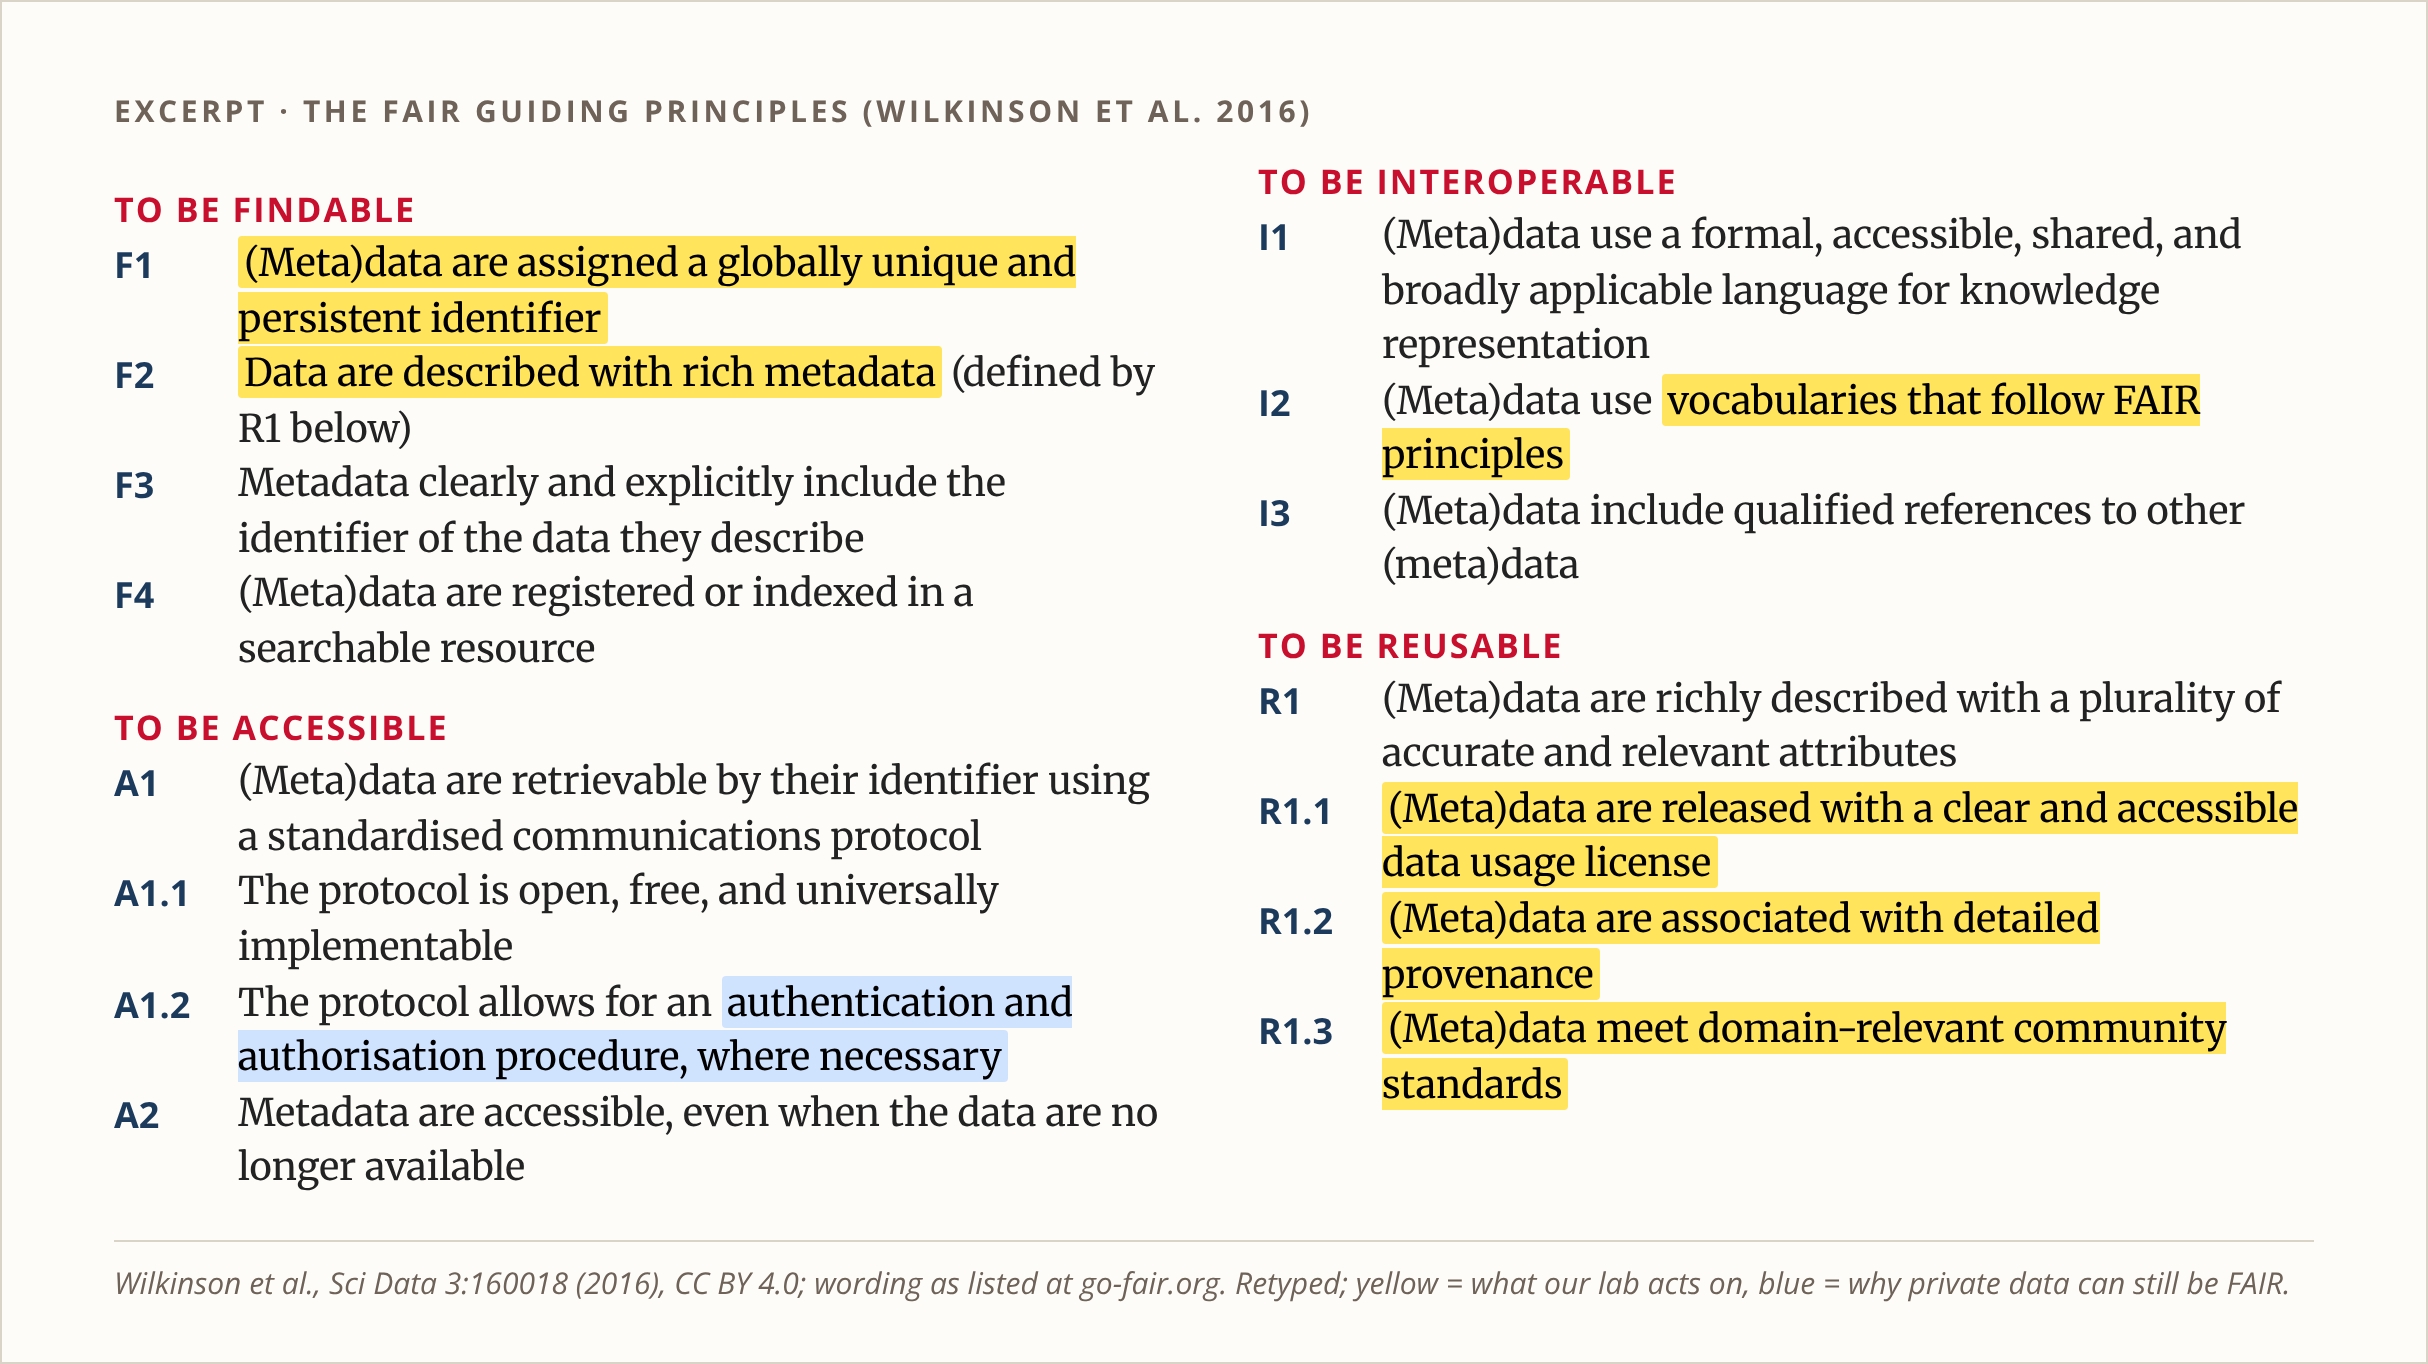
\includegraphics[width=6.44381in,height=3.62in]{img/excerpt_fair15.png}}}
\at{7.38381}{1.35}{\begin{minipage}[t]{1.92619in}\raggedright\fontsize{11}{14.3}\selectfont{}\color{isuBody}\par\vspace{5.5pt}{\color{isuNavy}\bfseries Repository gives us}\par\vspace{1pt}
F1 DOI, F4 indexing, A1–A2 access and long-lived metadata\par\vspace{3.3pt}
\par\vspace{5.5pt}{\color{isuNavy}\bfseries We must supply}\par\vspace{1pt}
F2/R1 rich metadata\par\vspace{3.3pt}
I2 shared trait terms\par\vspace{3.3pt}
R1.1 a license\par\vspace{3.3pt}
R1.2 provenance\par\vspace{3.3pt}
R1.3 MIAPPE / Croissant\par\vspace{3.3pt}
\par\vspace{5.5pt}{\color{isuNavy}\bfseries Blue = private is OK}\par\vspace{1pt}
A1.2 login and approval are allowed\par\vspace{3.3pt}\end{minipage}}
\note{Here are the actual 15 principles from the 2016 paper by Wilkinson and colleagues, retyped from the published list. You do not need to memorize them. Notice that about half are handled for us the moment we deposit data in a real repository: the DOI, the search index, the download protocol, and keeping the description online. The ones in yellow are our job, and the repository cannot do them for us: describe the data richly, use shared words for traits, pick a license, record how the data was made, and follow our field's standards, which for plant phenotyping is MIAPPE. The blue one, A1.2, is why private data can still be FAIR.}\end{frame}

\begin{frame}
\isutitle[21]{Written for machines, not only for people}
\at{1.4}{1.35}{\imgframe{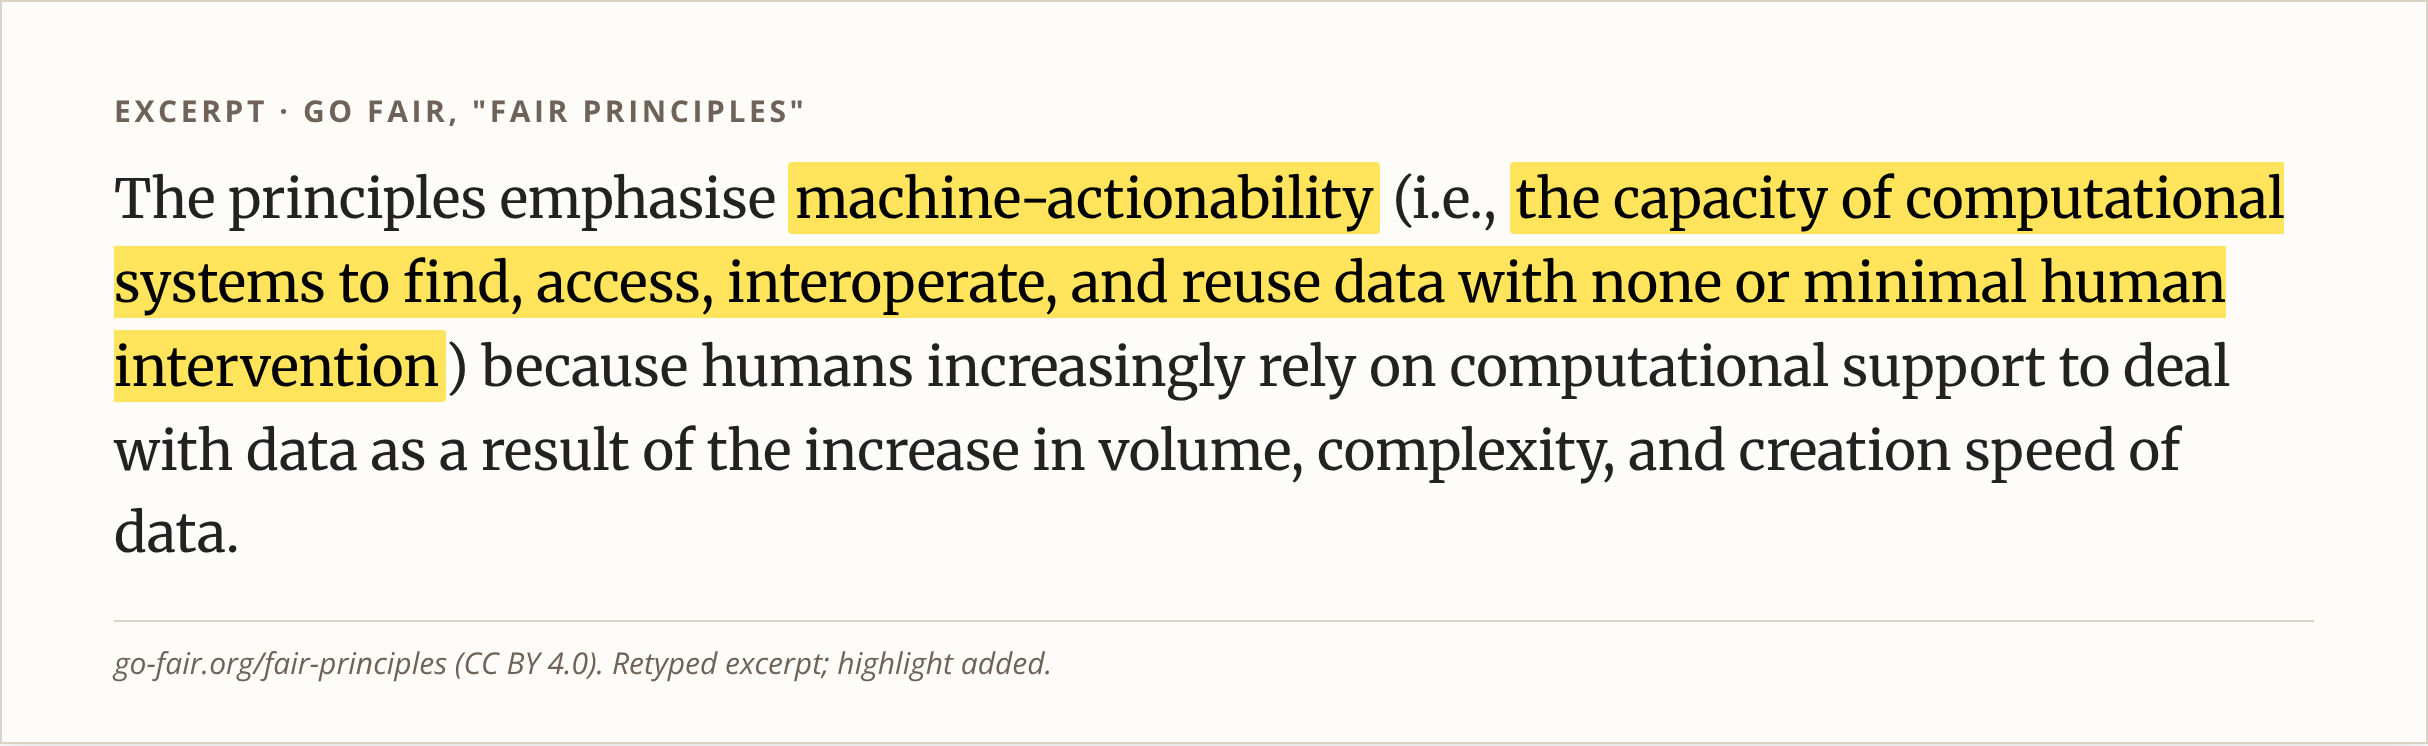
\includegraphics[width=7.2in,height=2.21219in]{img/excerpt_machine.png}}}
\panel{0.69}{3.72}{2.75}{1.3}{isuTintBlue}{\raggedright{\fontsize{12.5}{16.25}\selectfont{}\color{isuNavy}\bfseries Search engines}\par\vspace{3pt}{\fontsize{11}{14.3}\selectfont{}\color{isuBody}Google Dataset Search and repository search read structured metadata, not your README prose.}}
\panel{3.625}{3.72}{2.75}{1.3}{isuTintIce}{\raggedright{\fontsize{12.5}{16.25}\selectfont{}\color{isuNavy}\bfseries Scripts and pipelines}\par\vspace{3pt}{\fontsize{11}{14.3}\selectfont{}\color{isuBody}A loader can pull every LiDAR file from session 03 only if names and metadata follow a rule.}}
\panel{6.56}{3.72}{2.75}{1.3}{isuTintGreen}{\raggedright{\fontsize{12.5}{16.25}\selectfont{}\color{isuNavy}\bfseries AI agents}\par\vspace{3pt}{\fontsize{11}{14.3}\selectfont{}\color{isuBody}An agent can find, check, and load a Croissant-described dataset without emailing you.}}
\note{The principles have one unusual idea: they are written for computers as much as for people. The highlighted phrase says the goal is that software can find, access, combine, and reuse data with little or no human help. That is why a nice README in plain English is not enough. Search engines read structured metadata. Our own scripts can only grab, say, all the LiDAR from session three if the folders and names follow a rule. And AI agents, which many of us now use, can load a dataset described in Croissant without asking anyone. So the rules I show next are really about making our data machine-readable.}\end{frame}

\begin{frame}
\isutitle[18.5]{How to score it: one weak letter sinks the whole dataset}
\at{0.69}{1.33}{\begin{minipage}[t]{3.05in}\raggedright\fontsize{12}{15.6}\selectfont{}\color{isuBody}Score each of the 15 sub-principles 0, 0.5, or 1.\par\vspace{3.6pt}
\par\vspace{6pt}{\color{isuNavy}\bfseries Average}\par\vspace{1pt}
\par\vspace{2pt}{\color{isuInk}$\mathrm{FAIR\%}=\frac{100}{15}\sum_{k=1}^{15}s_k$}\par\vspace{2pt}
\par\vspace{6pt}{\color{isuNavy}\bfseries Weakest link (teaching model)}\par\vspace{1pt}
\par\vspace{2pt}{\color{isuInk}$P(\mathrm{reuse})\approx F\cdot A\cdot I\cdot R$}\par\vspace{2pt}
Reuse needs find AND open AND read AND trust, so the letters multiply.\par\vspace{3.6pt}
\par\vspace{6pt}{\color{isuNavy}\bfseries Our LiDAR example}\par\vspace{1pt}
Mean: {\color{isuInk}\bfseries 26.7\% $\rightarrow$ 93.3\%} (3.5$\times$)\par\vspace{3.6pt}
Product: {\color{isuInk}\bfseries 0.0026 $\rightarrow$ 0.729} (280$\times$)\par\vspace{3.6pt}\end{minipage}}
\at{3.95}{1.45}{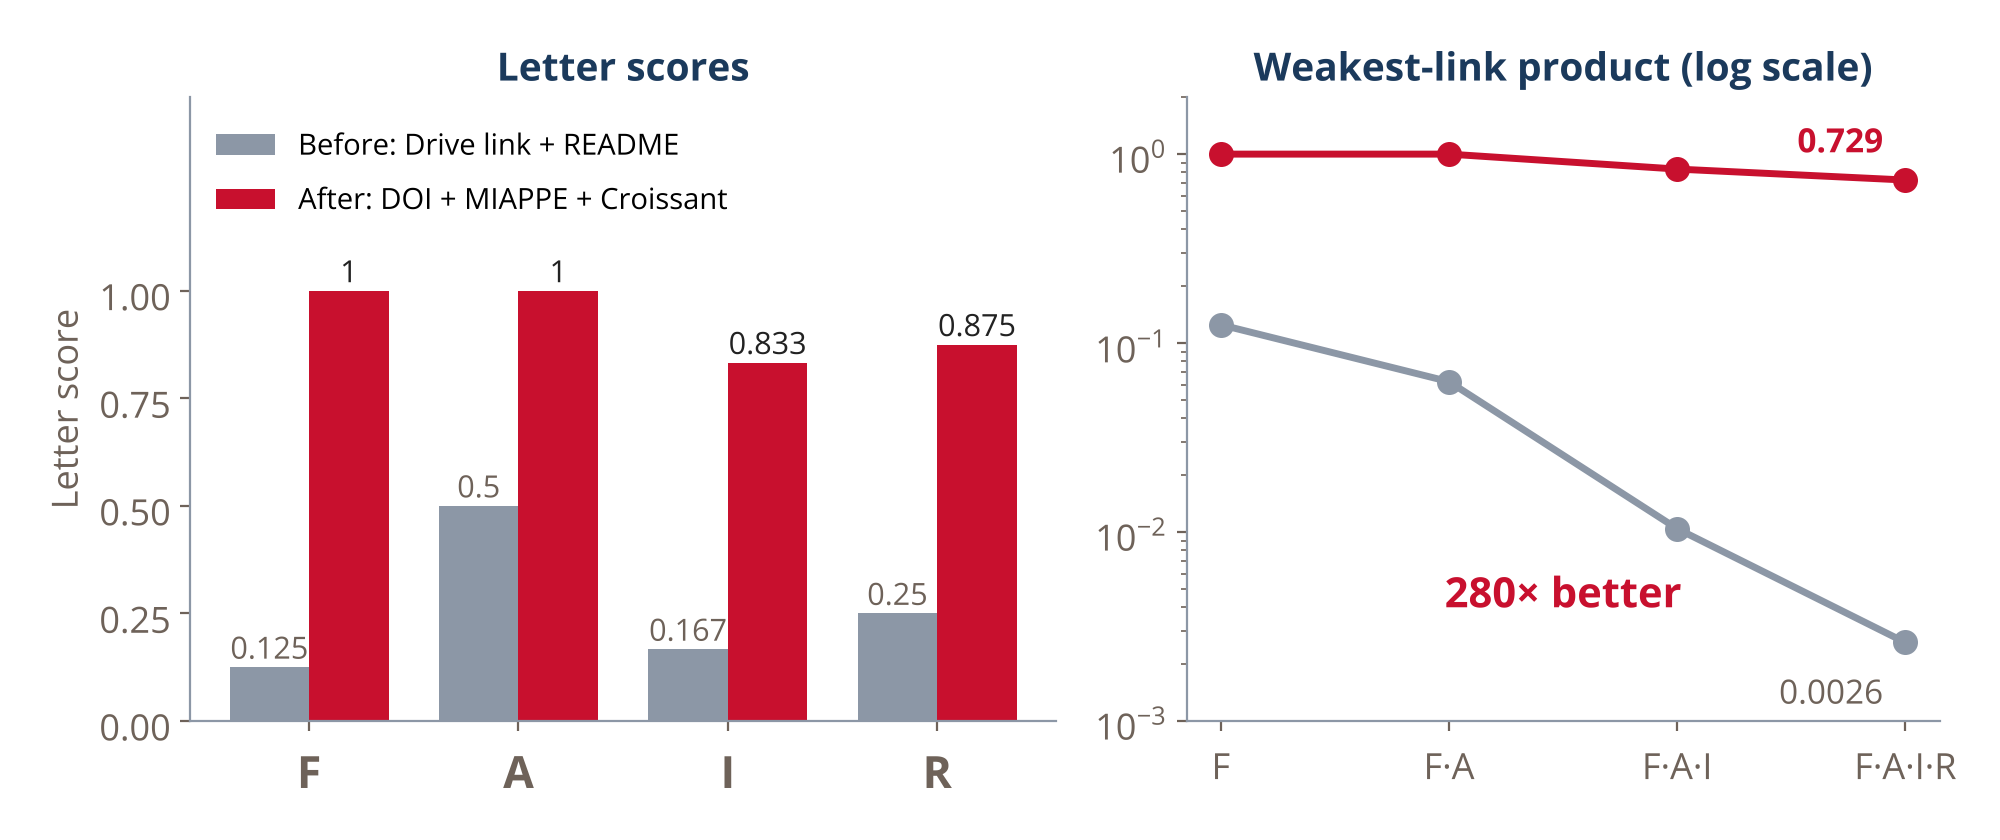
\includegraphics[width=5.36in,height=2.2512in]{img/fair_score_chart.png}}
\at{0.69}{5.08}{\fontsize{8}{10.4}\selectfont{}\color{isuCoolGray}Source: Worked example and scoring from our FAIR lesson; the product model is a teaching aid, not a published metric.}
\note{How do we know if we did a good job? Score each of the 15 sub-principles as zero, half, or one. The simple score is the average. But the average hides something. To reuse data, someone has to find it, and open it, and read it, and trust it. When steps are joined by AND, you multiply. So I also show the product of the four letter scores. For our LiDAR example, the folder on Google Drive scores 27 percent on average, which sounds bad but not hopeless. The product is 0.0026, which says almost nobody will ever reuse it. After we add a DOI, MIAPPE and Croissant metadata, and a license, the average is 93 percent and the product jumps 280 times. Lesson: fix your worst letter first. For most of us that is F, findable. This product is a teaching model, not an official metric.}\end{frame}

\begin{frame}
\isutitle[18.5]{Rule 1: one numbered folder layout for every project}
\panel{0.69}{1.4}{4.75}{3.6}{isuCode}{{\ttfamily\fontsize{10.5}{13.65}\selectfont{}\color{isuInk}maize-uav-lidar-2025/\\\hphantom{0}\hphantom{0}README.md\hphantom{0}\hphantom{0}\hphantom{0}\hphantom{0}\hphantom{0}\hphantom{0}\hphantom{0}\hphantom{0}\hphantom{0}\hphantom{0}\hphantom{0}\hphantom{0}$\leftarrow$\hphantom{0}start\hphantom{0}here\\\hphantom{0}\hphantom{0}00\_docs/\hphantom{0}\hphantom{0}\hphantom{0}\hphantom{0}\hphantom{0}\hphantom{0}\hphantom{0}\hphantom{0}\hphantom{0}\hphantom{0}\hphantom{0}\hphantom{0}\hphantom{0}notes,\hphantom{0}protocols\\\hphantom{0}\hphantom{0}01\_metadata/\hphantom{0}\hphantom{0}\hphantom{0}\hphantom{0}\hphantom{0}\hphantom{0}\hphantom{0}\hphantom{0}\hphantom{0}plot\hphantom{0}map,\hphantom{0}calibration,\\\hphantom{0}\hphantom{0}\hphantom{0}\hphantom{0}\hphantom{0}\hphantom{0}\hphantom{0}\hphantom{0}\hphantom{0}\hphantom{0}\hphantom{0}\hphantom{0}\hphantom{0}\hphantom{0}\hphantom{0}\hphantom{0}\hphantom{0}\hphantom{0}\hphantom{0}\hphantom{0}\hphantom{0}\hphantom{0}\hphantom{0}manifest,\hphantom{0}MIAPPE,\hphantom{0}Croissant\\\hphantom{0}\hphantom{0}02\_raw/\hphantom{0}\hphantom{0}\hphantom{0}\hphantom{0}\hphantom{0}\hphantom{0}\hphantom{0}\hphantom{0}\hphantom{0}\hphantom{0}\hphantom{0}\hphantom{0}\hphantom{0}\hphantom{0}straight\hphantom{0}off\hphantom{0}the\hphantom{0}sensor\\\hphantom{0}\hphantom{0}\hphantom{0}\hphantom{0}01\_uav\_rgb/01\_2025-07-14/\\\hphantom{0}\hphantom{0}\hphantom{0}\hphantom{0}04\_lidar/02\_2025-08-02/\\\hphantom{0}\hphantom{0}03\_processed/\hphantom{0}\hphantom{0}\hphantom{0}\hphantom{0}\hphantom{0}\hphantom{0}\hphantom{0}\hphantom{0}orthomosaics,\hphantom{0}clouds,\hphantom{0}3DGS\\\hphantom{0}\hphantom{0}04\_results/\hphantom{0}\hphantom{0}\hphantom{0}\hphantom{0}\hphantom{0}\hphantom{0}\hphantom{0}\hphantom{0}\hphantom{0}\hphantom{0}trait\hphantom{0}tables,\hphantom{0}models\\\hphantom{0}\hphantom{0}05\_code/\hphantom{0}\hphantom{0}\hphantom{0}\hphantom{0}\hphantom{0}\hphantom{0}\hphantom{0}\hphantom{0}\hphantom{0}\hphantom{0}\hphantom{0}\hphantom{0}\hphantom{0}scripts,\hphantom{0}git\hphantom{0}commit\\\hphantom{0}\hphantom{0}99\_review/\hphantom{0}\hphantom{0}\hphantom{0}\hphantom{0}\hphantom{0}\hphantom{0}\hphantom{0}\hphantom{0}\hphantom{0}\hphantom{0}\hphantom{0}possible\hphantom{0}duplicates}}
\at{5.65}{1.4}{\begin{minipage}[t]{3.66in}\raggedright\fontsize{12}{15.6}\selectfont{}\color{isuBody}\par\vspace{6pt}{\color{isuNavy}\bfseries Read the numbers in order}\par\vspace{1pt}
00 $\rightarrow$ 05 is the path a new student should follow: what it is, how to read it, the data, what we made from it, and the code.\par\vspace{3.6pt}
\par\vspace{6pt}{\color{isuNavy}\bfseries Inside each folder}\par\vspace{1pt}
Data types are numbered in {\color{isuInk}\bfseries pipeline order}: sensor data before the products made from it.\par\vspace{3.6pt}
\par\vspace{6pt}{\color{isuNavy}\bfseries Raw is read-only}\par\vspace{1pt}
Never edit files in 02\_raw. Everything else can be rebuilt from raw + code.\par\vspace{3.6pt}\end{minipage}}
\note{Rule one is a single folder layout for every project. The numbers are the reading order for someone new. Zero zero is docs: what is this. Zero one is metadata: the plot map and calibration you need to make sense of anything else. Zero two is raw data straight off each sensor. Zero three is what we processed from it. Zero four is the final results that go into papers. Zero five is the code. Inside each folder, data types are numbered in pipeline order. And one hard rule: never edit anything in raw. If processed data is lost, we can rebuild it from raw plus code. If raw is changed, we cannot.}\end{frame}

\begin{frame}
\isutitle[18.5]{Rule 2: names carry the date, the session, and nothing else}
\at{0.69}{1.33}{\begin{minipage}[t]{8.62in}\raggedright\fontsize{12}{15.6}\selectfont{}\color{isuBody}\begin{itemize}\setlength{\itemsep}{3.6pt}\setlength{\leftmargini}{1.1em}
\item Dates in ISO 8601: {\color{isuInk}\bfseries 2025-07-14} in folders, {\color{isuInk}\bfseries 20250714} in names, so they sort in time order.
\item Each field day gets one {\color{isuInk}\bfseries session number} shared by every sensor: s01 = 2025-07-14 for drone, LiDAR, and photos.
\item No spaces, and no {\color{isuInk}\bfseries final}, {\color{isuInk}\bfseries v3}, {\color{isuInk}\bfseries REAL}, or {\color{isuInk}\bfseries copy}. Versions live in git or the README.
\item Keep sensor timestamp names (DJI\_2025…); rename only meaningless ones (IMG\_4521, Untitled1).
\end{itemize}\end{minipage}}
\at{0.69}{2.95}{{\fontsize{9.5}{12.35}\selectfont{}\renewcommand{\arraystretch}{1.3}\setlength{\tabcolsep}{0.06in}\arrayrulecolor{isuTintBlue}\begin{tabular}{>{\raggedright\arraybackslash}p{3.48in}>{\raggedright\arraybackslash}p{4.9in}}\rowcolor{isuNavy}\textcolor{white}{\bfseries Before} & \textcolor{white}{\bfseries After}\\
\rowcolor{white}\textcolor{isuNavy}{flight july 14/DJI\_20250714101502\_0001\_D.JPG} & 02\_raw/01\_uav\_rgb/01\_2025-07-14/DJI\_20250714101502\_0001\_D.jpg\\
\rowcolor{isuCode}\textcolor{isuNavy}{lidar/lidar\_aug2\_v3\_REAL (1).laz} & 99\_review/duplicates/…/lidar\_aug2\_v3.laz\\
\rowcolor{white}\textcolor{isuNavy}{misc/New folder/IMG\_4521.HEIC} & 02\_raw/06\_photos/01\_2025-07-14/s01\_20250714\_aea\_photos\_0001.heic\\
\rowcolor{isuCode}\textcolor{isuNavy}{notes/plot map FINAL.xlsx} & 01\_metadata/01\_field\_design/plot\_map.xlsx\\\end{tabular}}}
\note{Rule two is about names. Dates always go year, month, day, so files sort in time order on any computer. Each field day gets one session number, and that number is the same for every sensor, so session one means July fourteenth whether you are looking at drone photos or LiDAR. No spaces, and never final, v3, REAL, or copy in a name: that is what version control and the README are for. Keep names that already carry meaning, like the DJI timestamp names. Only rename meaningless ones like IMG underscore four five two one. The table shows real examples from our demo folder. You will not do this by hand; the tool on the next slides does it.}\end{frame}

\begin{frame}
\isutitle[18.5]{Rule 3: open formats, plus the context that must travel with them}
\at{0.69}{1.38}{{\fontsize{10.5}{13.65}\selectfont{}\renewcommand{\arraystretch}{1.3}\setlength{\tabcolsep}{0.06in}\arrayrulecolor{isuTintBlue}\begin{tabular}{>{\raggedright\arraybackslash}p{1.63in}>{\raggedright\arraybackslash}p{1.98in}>{\raggedright\arraybackslash}p{4.65in}}\rowcolor{isuNavy}\textcolor{white}{\bfseries Data} & \textcolor{white}{\bfseries Format} & \textcolor{white}{\bfseries Must travel with it}\\
\rowcolor{white}\textcolor{isuNavy}{UAV images} & JPG / TIFF / DNG & EXIF + GPS kept, flight and RTK logs, calibration panel\\
\rowcolor{isuCode}\textcolor{isuNavy}{LiDAR} & LAS / LAZ & CRS (EPSG code) in the header, processing software and version\\
\rowcolor{white}\textcolor{isuNavy}{Hyperspectral} & ENVI .hdr + .bil & Wavelength list, white and dark references\\
\rowcolor{isuCode}\textcolor{isuNavy}{3D (SfM / NeRF / 3DGS)} & PLY + transforms.json & Camera poses, training settings, code commit\\
\rowcolor{white}\textcolor{isuNavy}{Genotypes} & VCF (.vcf.gz) & Reference genome version (e.g. B73 v5)\\
\rowcolor{isuCode}\textcolor{isuNavy}{Traits} & CSV / Parquet & Units and Crop Ontology trait IDs\\\end{tabular}}}
\panel{0.69}{4.08}{2.75}{0.95}{isuTintBlue}{\raggedright{\fontsize{12}{15.6}\selectfont{}\color{isuNavy}\bfseries MIAPPE 1.1}\par\vspace{3pt}{\fontsize{10.5}{13.65}\selectfont{}\color{isuBody}Describes the experiment: site, design, plants, traits.}}
\panel{3.625}{4.08}{2.75}{0.95}{isuTintIce}{\raggedright{\fontsize{12}{15.6}\selectfont{}\color{isuNavy}\bfseries Croissant}\par\vspace{3pt}{\fontsize{10.5}{13.65}\selectfont{}\color{isuBody}Describes an ML-ready dataset in JSON-LD.}}
\panel{6.56}{4.08}{2.75}{0.95}{isuTintGreen}{\raggedright{\fontsize{12}{15.6}\selectfont{}\color{isuNavy}\bfseries Crop Ontology}\par\vspace{3pt}{\fontsize{10.5}{13.65}\selectfont{}\color{isuBody}Shared IDs so "plant height" means one thing.}}
\note{Rule three: use open formats, and keep the context that makes them readable. A LiDAR file without its coordinate system is a cloud of meaningless numbers. A hyperspectral cube without its wavelength list cannot be compared to anything. A Gaussian splat without camera poses and settings cannot be reproduced. So for each data type, this table lists the format and what must travel with it. On top of that we use three community standards: MIAPPE to describe the plant experiment, Croissant to describe a dataset for machine learning, and Crop Ontology so a trait like plant height has one agreed definition and ID.}\end{frame}

\begin{frame}
\isutitle[21]{Demo: FAIR Folder Curator reads the messy folder}
\at{0.69}{1.35}{\imgframe{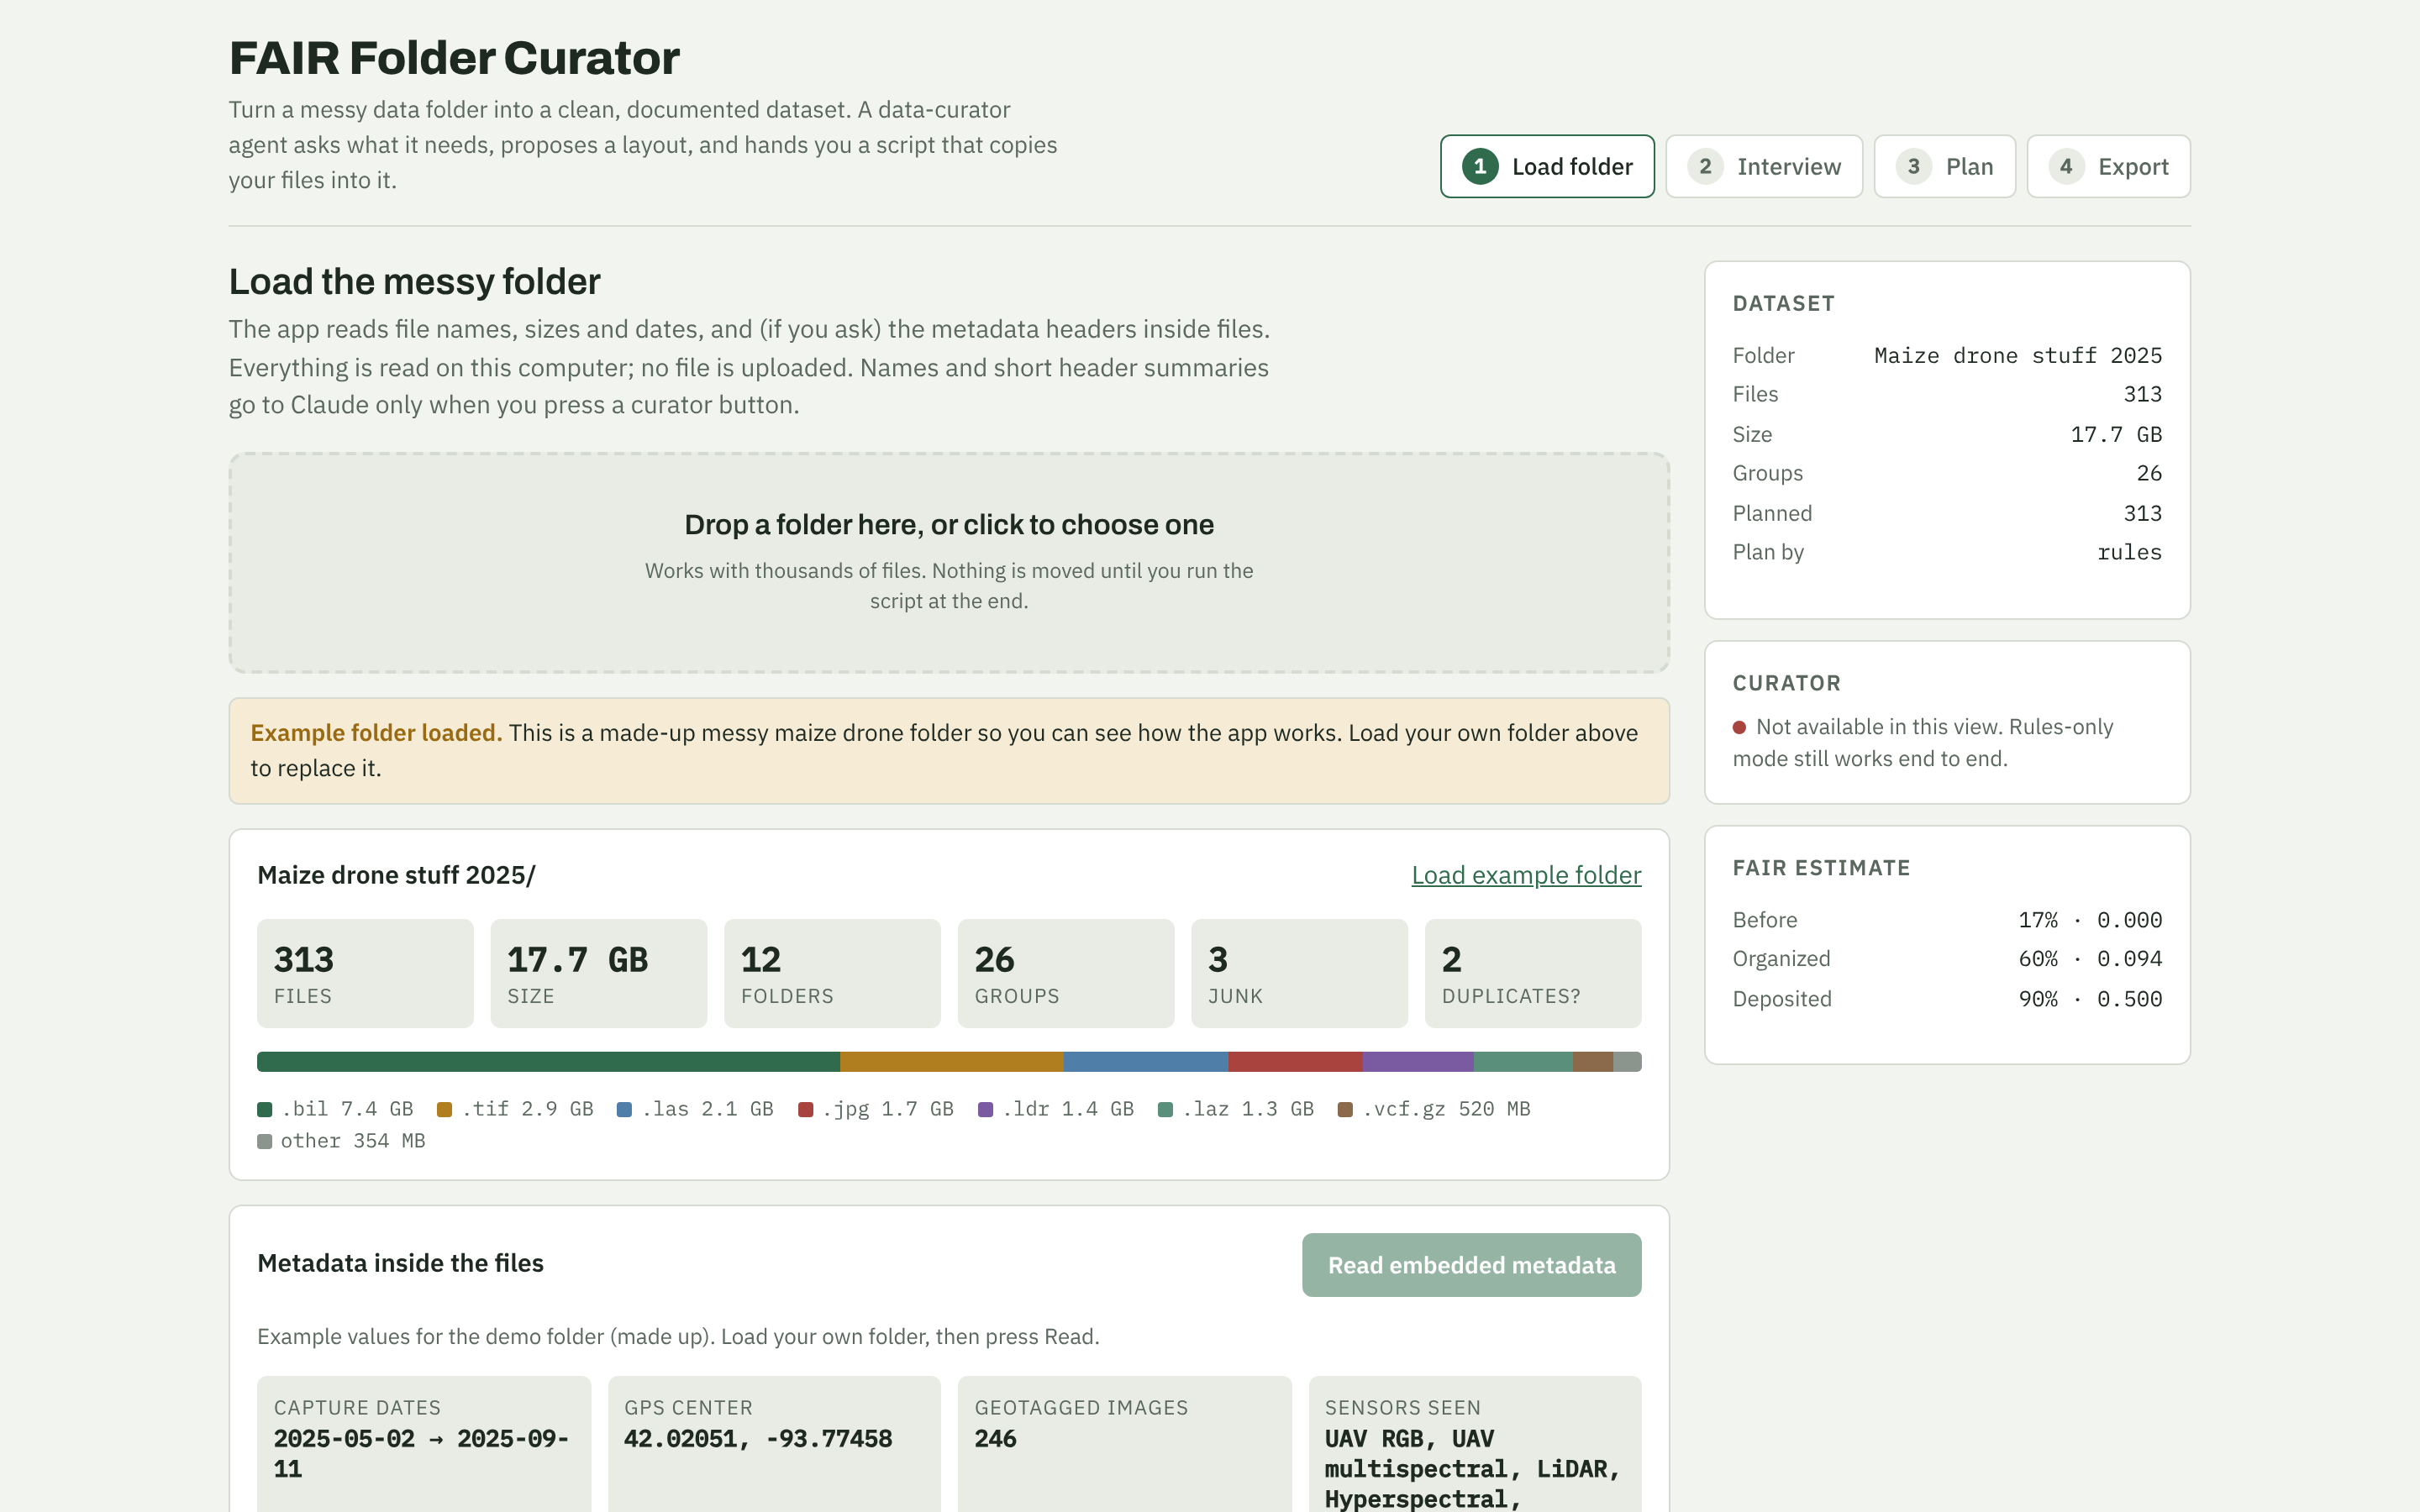
\includegraphics[width=4.72in,height=2.95in]{img/app_step1.png}}}
\at{6.0718}{1.35}{\imgframe{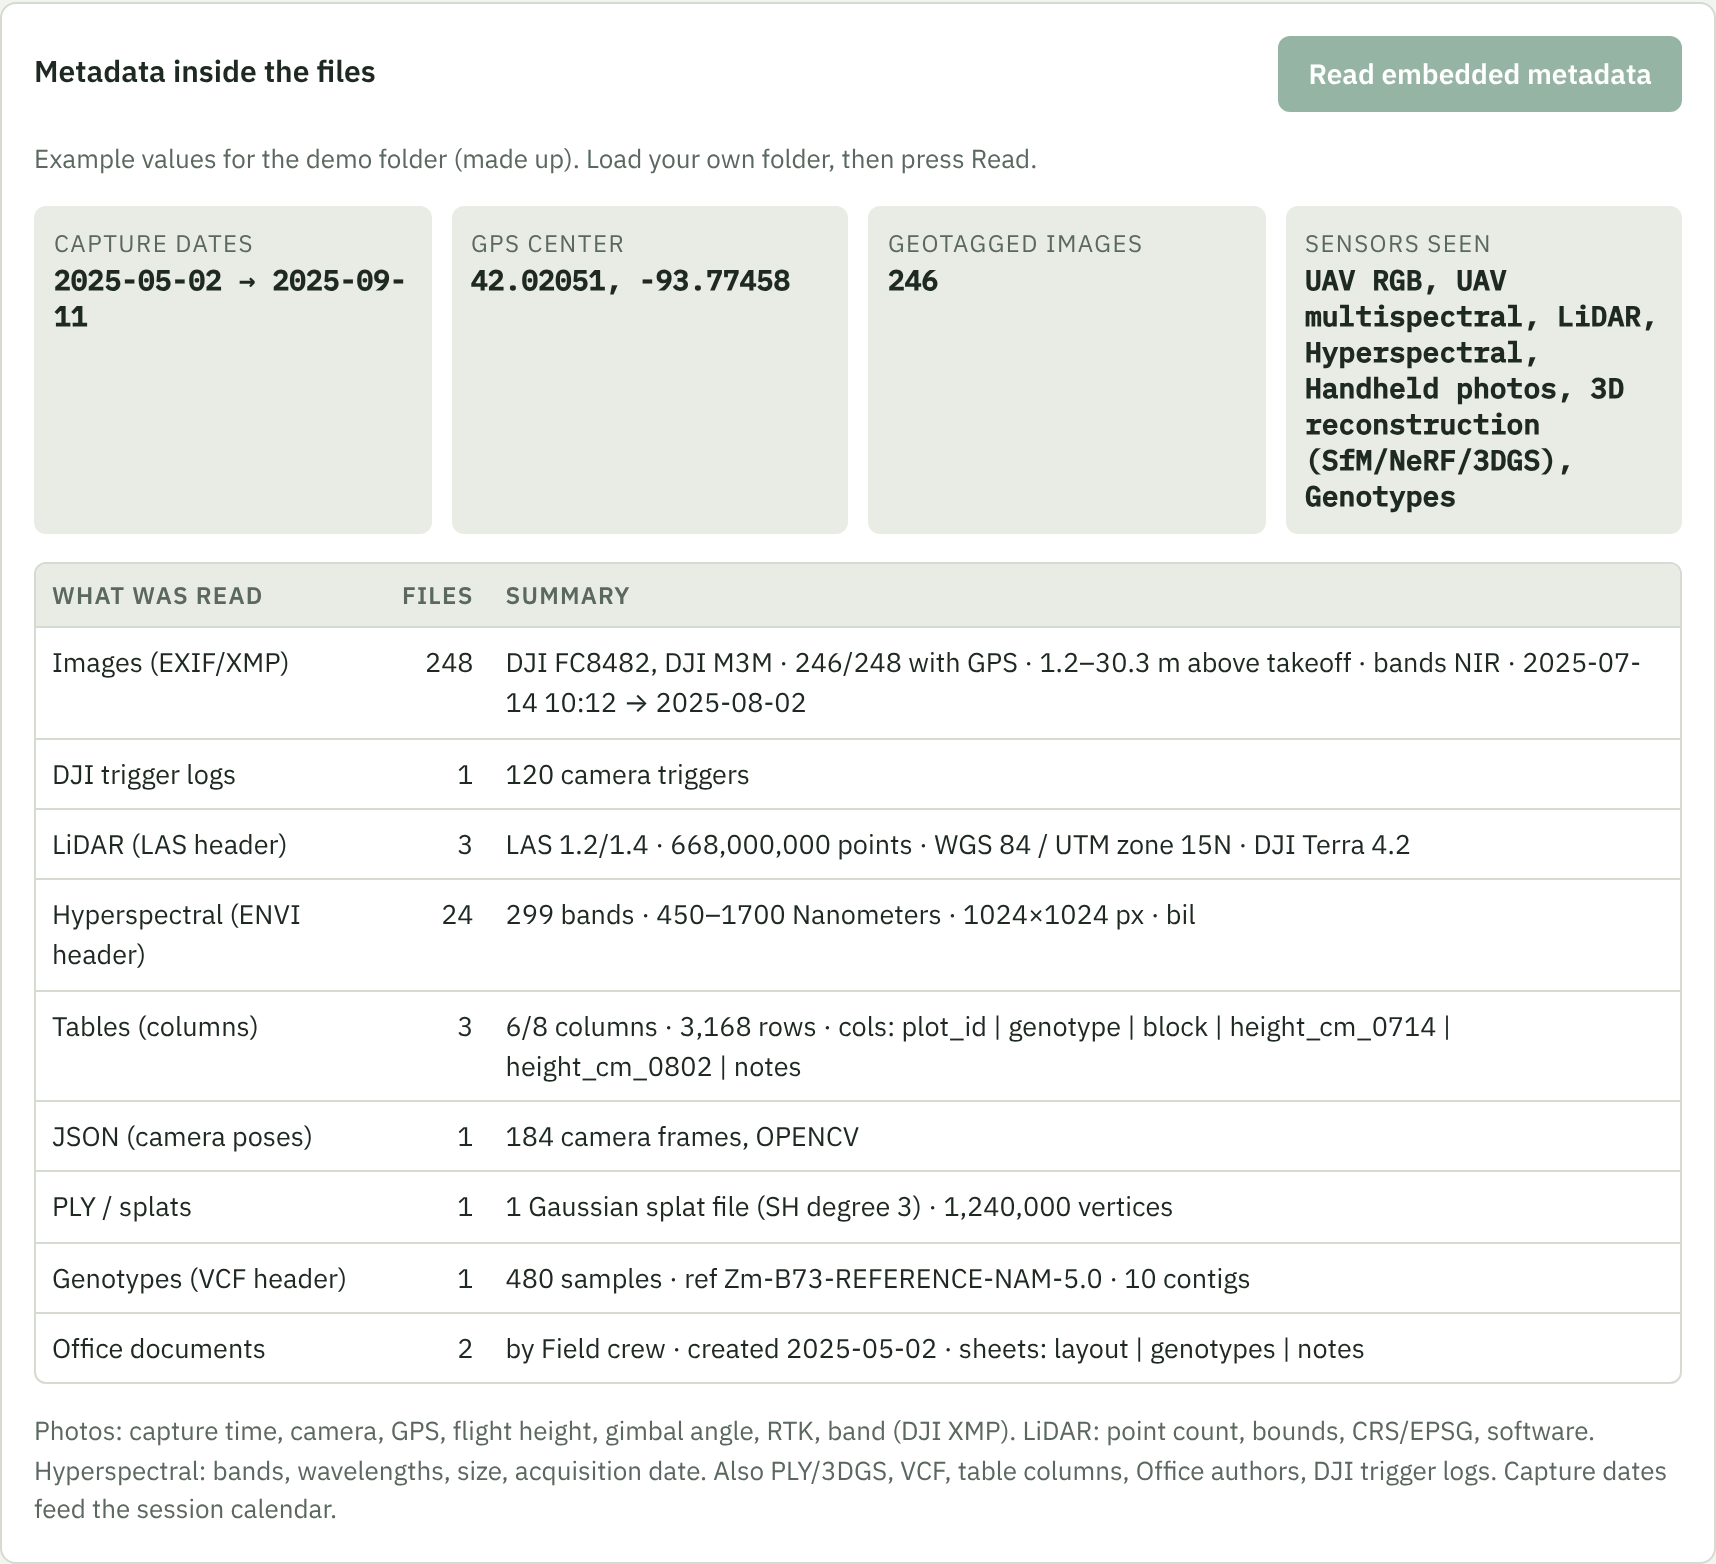
\includegraphics[width=3.2367in,height=2.95in]{img/app_meta.png}}}
\at{0.69}{4.42}{\begin{minipage}[t]{8.62in}\raggedright\fontsize{11.5}{14.95}\selectfont{}\color{isuBody}Drop a folder in. It reads names, sizes, dates, and file headers (GPS, capture time, LiDAR CRS, band lists) {\color{isuInk}\bfseries on your computer; nothing is uploaded}. A data-curator agent then asks 3–7 questions about what it cannot see.\par\vspace{3.45pt}\end{minipage}}
\note{Doing all of this by hand is boring, so I built a tool. It is a web page called FAIR Folder Curator. You drop a messy folder into it. It reads only file names, sizes, dates, and the metadata stored inside files, like GPS and capture time from drone photos, the coordinate system from LiDAR, and the wavelength list from hyperspectral headers. Everything is read on your own computer; nothing is uploaded. Then a curator agent asks a few questions about what it cannot see, such as which files are raw and which are processed. This screen is the built-in example folder, which is made up.}\end{frame}

\begin{frame}
\isutitle[18.5]{Demo: it plans the layout and hands you a safe script}
\at{0.69}{1.38}{\imgframe{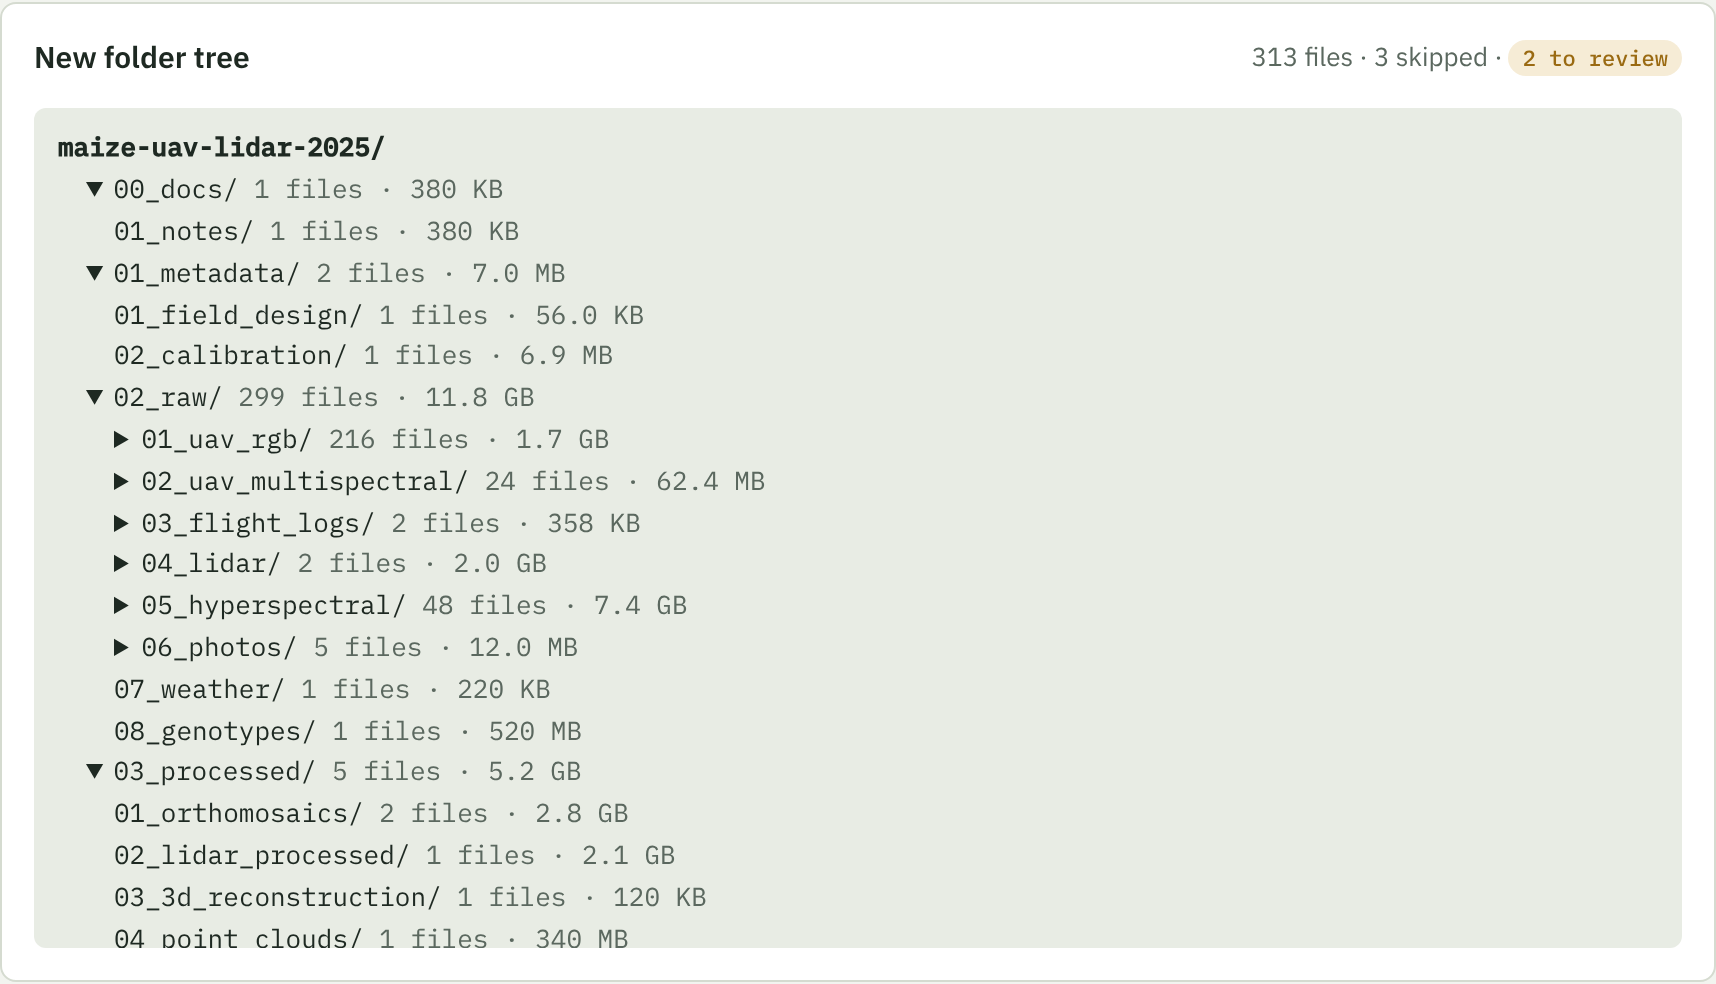
\includegraphics[width=4.2in,height=2.40839in]{img/app_tree.png}}}
\at{5.1}{1.38}{\imgframe{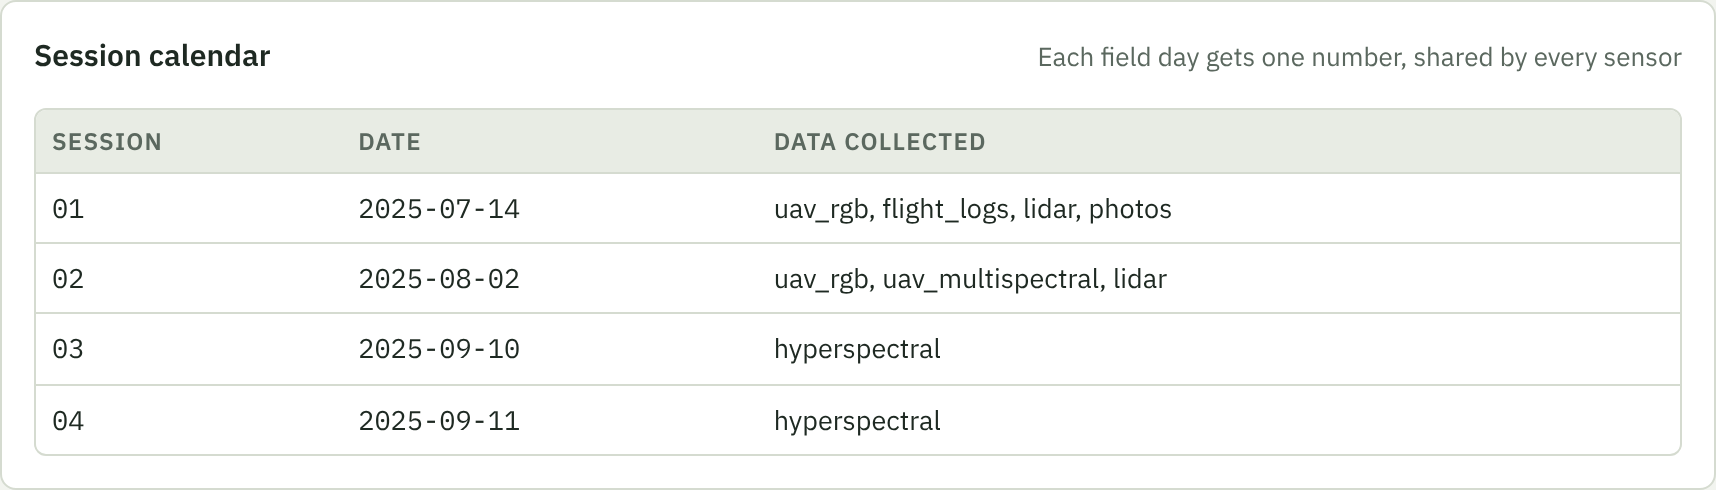
\includegraphics[width=4.21in,height=1.20216in]{img/app_sessions.png}}}
\panel{5.1}{2.75}{4.21}{1.25}{isuCode}{{\ttfamily\fontsize{9}{11.7}\selectfont{}\color{isuInk}{\color{isuCoolGray}\#\hphantom{0}1.\hphantom{0}preview:\hphantom{0}changes\hphantom{0}nothing}\\python\hphantom{0}organize.py\hphantom{0}"messy"\hphantom{0}"clean"\\{\color{isuCoolGray}\#\hphantom{0}2.\hphantom{0}copy\hphantom{0}into\hphantom{0}the\hphantom{0}new\hphantom{0}layout}\\python\hphantom{0}organize.py\hphantom{0}"messy"\hphantom{0}"clean"\hphantom{0}--apply\\{\color{isuCoolGray}\#\hphantom{0}3.\hphantom{0}changed\hphantom{0}your\hphantom{0}mind?}\\python\hphantom{0}organize.py\hphantom{0}--undo\hphantom{0}clean/01\_metadata/manifest.csv}}
\at{5.1}{4.1}{\begin{minipage}[t]{4.21in}\raggedright\fontsize{11}{14.3}\selectfont{}\color{isuBody}\begin{itemize}\setlength{\itemsep}{3.3pt}\setlength{\leftmargini}{1.1em}
\item Copies by default; your originals stay put.
\item manifest.csv maps every old path to its new one.
\item Also writes README, MIAPPE, Croissant, FAIR report.
\end{itemize}\end{minipage}}
\note{After the interview, the tool proposes the numbered layout you saw earlier, with a session calendar so everyone knows that session one is July fourteenth. You can edit any of it. Then it gives you a small Python script. Run it once and it only shows you what it would do. Add dash dash apply and it copies everything into the new layout, leaving your originals alone. It writes a manifest that maps every old path to its new one, so dash dash undo can reverse it. It also writes the README, the MIAPPE sheet, the Croissant file, and a FAIR score report.}\end{frame}

\begin{frame}
\isutitle[21]{Last mile: license, deposit, check, cite}
\at{0.69}{1.35}{\begin{minipage}[t]{4.6in}\raggedright\fontsize{11.5}{14.95}\selectfont{}\color{isuBody}\par\vspace{5.75pt}{\color{isuNavy}\bfseries License}\par\vspace{1pt}
CC BY 4.0 for data, MIT for code. No license means nobody may legally reuse it.\par\vspace{3.45pt}
\par\vspace{5.75pt}{\color{isuNavy}\bfseries Deposit (this gives the DOI)}\par\vspace{1pt}
ISU DataShare · Zenodo · CyVerse Data Commons · Hugging Face (ML sets) · NCBI SRA (reads)\par\vspace{3.45pt}
\par\vspace{5.75pt}{\color{isuNavy}\bfseries Check}\par\vspace{1pt}
Run the DOI through {\color{isuInk}\bfseries F-UJI}, a free automated FAIR checker; fix what fails.\par\vspace{3.45pt}
\par\vspace{5.75pt}{\color{isuNavy}\bfseries Cite}\par\vspace{1pt}
Put the DOI in the paper's data-availability statement. Papers linking data in a repository saw up to {\color{isuInk}\bfseries 25\% more citations} (an association, not proof).\par\vspace{3.45pt}\end{minipage}}
\at{5.5}{1.38}{\imgframe{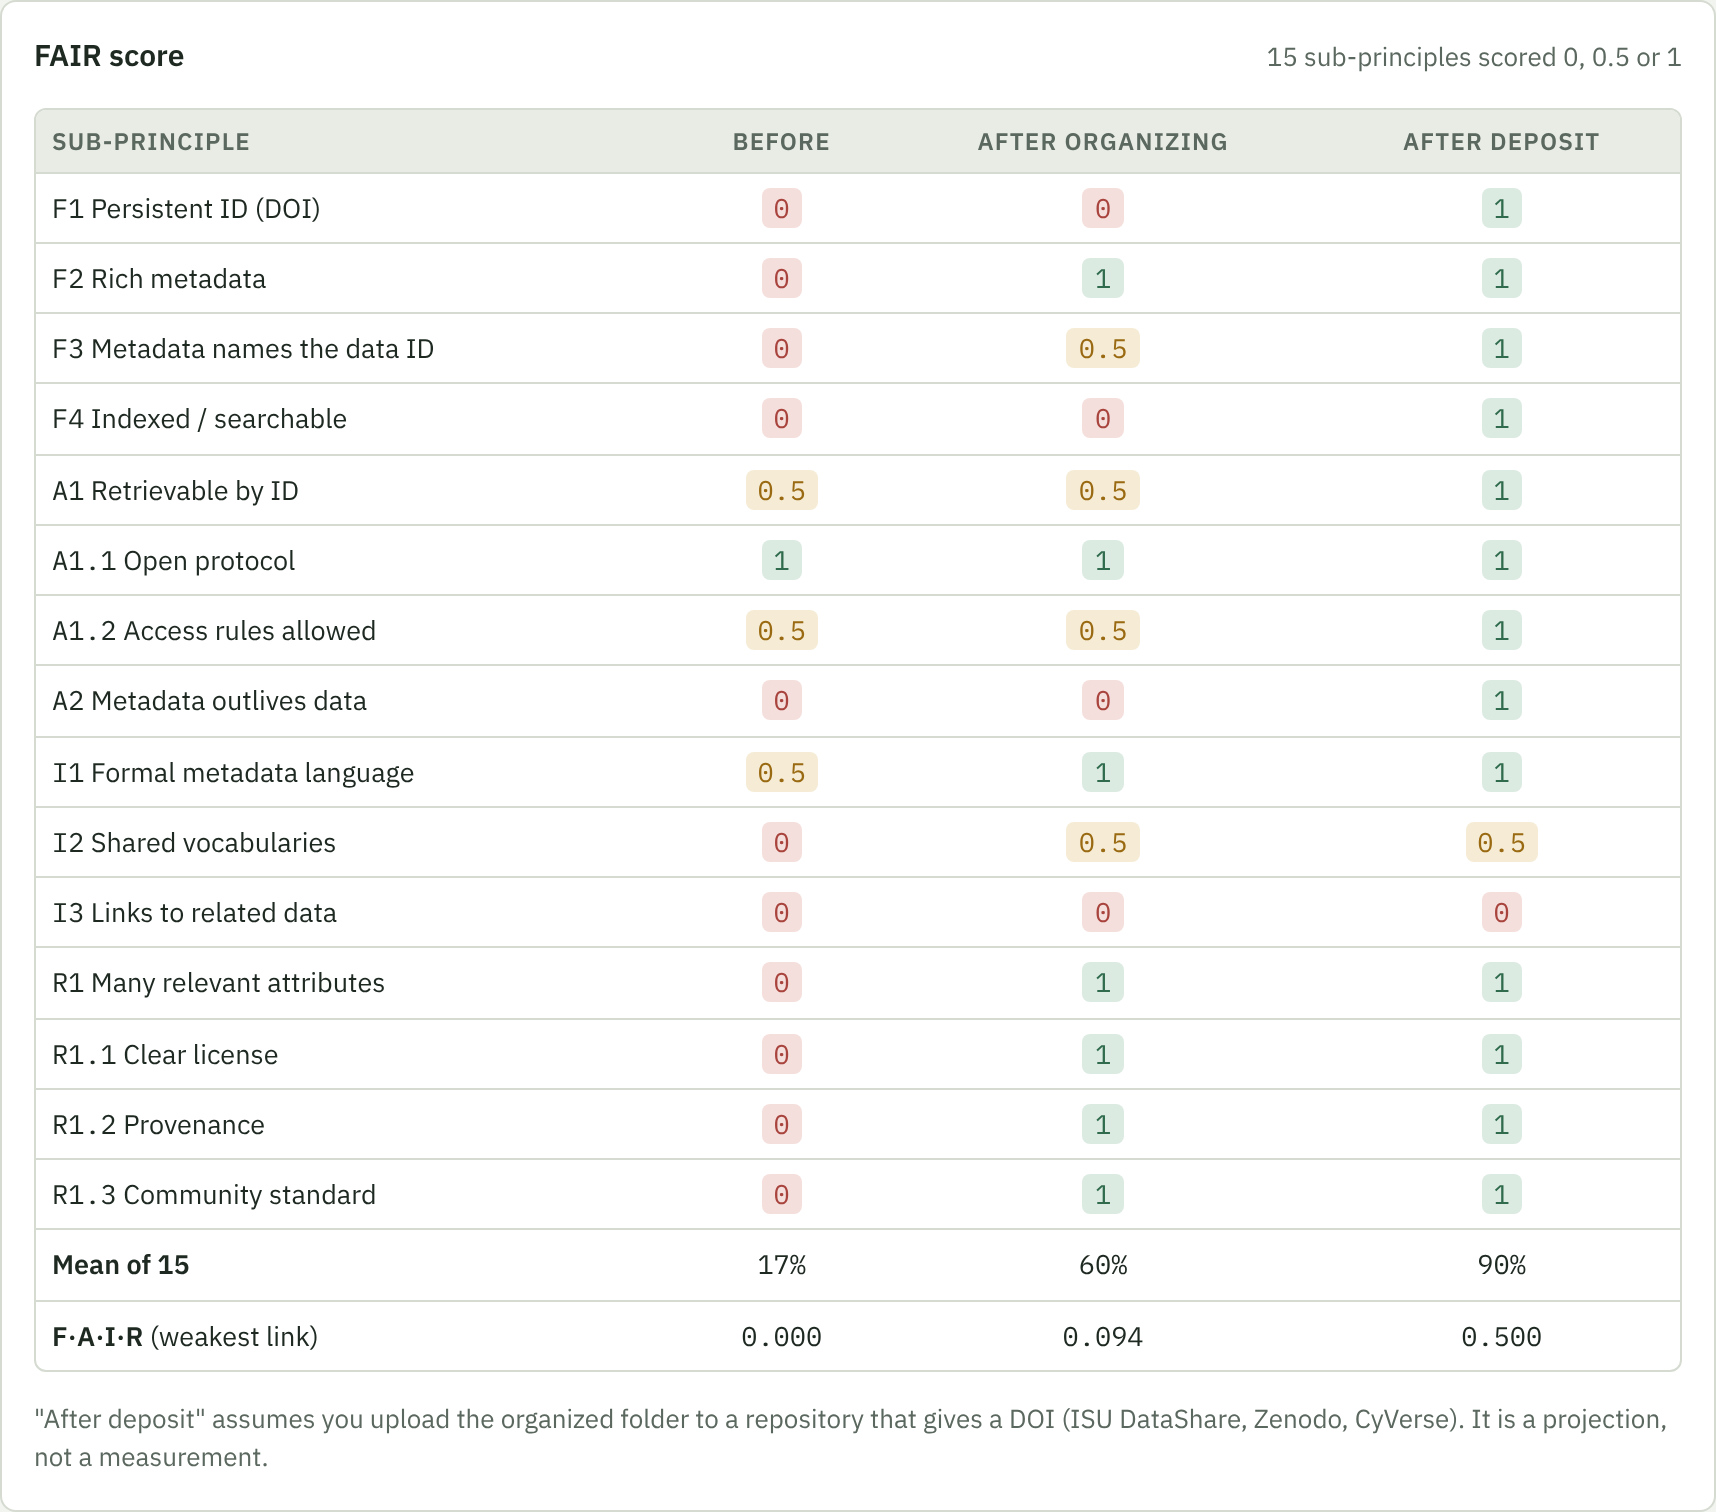
\includegraphics[width=4.10841in,height=3.62in]{img/app_fair.png}}}
\at{0.69}{5.08}{\fontsize{8}{10.4}\selectfont{}\color{isuCoolGray}Source: Colavizza et al., PLOS ONE 2020; Devaraju \& Huber, Patterns 2021 (F-UJI).}
\note{Organizing the folder gets us about halfway. The last mile is four steps. Pick a license: CC BY for data and MIT for code are the usual choices; with no license, nobody may legally reuse the data. Deposit it in a repository that gives a DOI; ISU DataShare, Zenodo, and CyVerse all work, and Hugging Face is good for machine-learning datasets. Check it with F-UJI, a free tool that tests a DOI against the FAIR principles. And cite the DOI in your paper. A large study of PLOS and BMC papers found that papers linking their data in a repository got up to a quarter more citations. That is a correlation, not proof, but it points the right way. On the right is the tool's own score table: after organizing, then projected after deposit.}\end{frame}

\begin{frame}
\isutitle[21]{Your job before next group meeting}
\at{0.69}{1.4}{\begin{minipage}[t]{5.1in}\raggedright\fontsize{14}{18.2}\selectfont{}\color{isuBody}\begin{itemize}\setlength{\itemsep}{4.2pt}\setlength{\leftmargini}{1.1em}
\item {\color{isuInk}\bfseries Pick} one dataset you own.
\item {\color{isuInk}\bfseries Run} it through FAIR Folder Curator and answer the interview.
\item {\color{isuInk}\bfseries Preview}, then {\color{isuInk}\bfseries --apply} organize.py (it copies; originals stay).
\item {\color{isuInk}\bfseries Fill} the README blanks: processing steps, license, trait IDs.
\item {\color{isuInk}\bfseries Bring} your before and after FAIR score.
\end{itemize}\end{minipage}}
\panel{6.05}{1.4}{3.26}{2.95}{isuTintBlue}{\raggedright{\fontsize{12.5}{16.25}\selectfont{}\color{isuNavy}\bfseries Everything is in one repo}\par\vspace{3pt}{\fontsize{11}{14.3}\selectfont{}\color{isuBody}github.com/znjubery/fair-data-curation\par \vspace{2pt}\par This talk (PPTX, Beamer, PDF), the Folder Curator app, the FAIR lesson, and the excerpt images.}}
\statement{0.69}{4.45}{8.62}{0.6}{\fontsize{13}{16.9}\selectfont{}{\color{isuInk}\bfseries FAIR in one line:} a stranger, or a script, can find, open, understand, and legally reuse your data without emailing you.}
\note{Here is the homework. Pick one dataset you own. Put it through the tool and answer its questions. Preview, then apply the script. Fill in the blanks in the README it writes: processing steps, license, trait IDs. And bring your before and after score to the next group meeting so we can compare. Everything from today is in one GitHub repository. If you remember one line, remember this: FAIR means a stranger, or a script, can find, open, understand, and legally reuse your data without emailing you.}\end{frame}

\end{document}